\section{Progettazione logica}

\subsection{Analisi delle ridondanze}
Nello schema concettuale possiamo individuare stato di occupazione che è attributo di molo e deducibile dalla relazione sosta, la quale presenta l'attributo data di arrivo e data di partenza.

Le operazioni coinvolte sono la numero 3 e la numero 6 che presentano una frequenza di 40 volte al giorno e 30-40 volte ogni giorno.

Si procede alla valutazione del costo totale in termini di accessi nel caso di ridondanza e di assenza di essa.

\begin{center}
    \begin{tabularx}{\textwidth}{|p{90mm}|X|}
        \hline
        \rowcolor{gray!30}
        \textbf{Operazione} & \textbf{Frequenza}\\
        \hline
        3. Controllo dei posti disponibili per una certa imbarcazione(Controllo delle dimensioni)& 40 volte al giorno\\
        \hline
        6. Arrivo di un'imbarcazione nel marina & 30-40 volte al giorno\\
        \hline
    \end{tabularx}
\end{center}

Ci riferiremo per i nostri calcoli a dei volumi plausibili nella vita della base di dati. I moli non variano particolarmente di numero, le imbarcazioni vengono registrate al loro primo accesso e le soste aumentano ogni giorno. Mediamente un'imbarcazione sosta 2,7 volte in un molo.

\begin{center}
    \begin{tabularx}{\textwidth}{|X|X|X|}
        \hline
        \rowcolor{gray!30}
        \textbf{Concetto} & \textbf{Tipo} & \textbf{Volume}\\
        \hline
        Molo & ENTITÀ & 250\\
        \hline
        Imbarcazione & ENTITÀ & 5000\\
        \hline
        Sosta & ENTITÀ & 13500\\ % Contando che ogni imbarcazione sosta in media due volte per molo.
        \hline
        M\_S & RELAZIONE & 13500\\ % Contando che ogni imbarcazione sosta in media due volte per molo.
        \hline
    \end{tabularx}
\end{center}

\paragraph{operazione 3}

\begin{center}
    \begin{minipage}{.48\linewidth}
        \begin{tabularx}{\linewidth}{|X|l|l|l|}
            \hline
            \rowcolor{gray!30}
            \multicolumn{4}{|c|}{\textbf{Con ridondanza}}\\
            \hline
            \rowcolor{gray!15}
            Concetto & Costrutto & Accessi & Tipo\\
            \hline
            Molo & E & 250 & L\\
            \hline
        \end{tabularx}
    \end{minipage}
    \begin{minipage}{.48\linewidth}
        \begin{tabularx}{\linewidth}{|X|l|l|l|}
            \hline
            \rowcolor{gray!30}
            \multicolumn{4}{|c|}{\textbf{Senza ridondanza}}\\
            \hline
            \rowcolor{gray!15}
            Concetto & Costrutto & Accessi & Tipo\\
            \hline
            Sosta & E & 13500 & L\\
            \hline
            M\_S & R & 13500 & L\\
            \hline
            Molo & E & 250 & L\\
            \hline
        \end{tabularx}
    \end{minipage}
\end{center}

\underline{Con ridondanza}
\begin{itemize}
    \item Totale accessi(Solo in lettura): $250\xrightarrow{*40} 10000$
\end{itemize}

\underline{Senza ridondanza}
\begin{itemize}
    \item Totale accessi(Solo in lettura): $250+13500+13500 = 27250 \xrightarrow{*40} 1090000$ Giornalieri
\end{itemize}

\paragraph{operazione 6}

Assumo che l'imbarcazione sia già presente perché l'esserci o non esserci non cambia il calcolo della ridondanza.

\begin{center}
\begin{tabularx}{\linewidth}{|X|}
    \hline
    \rowcolor{gray!30}
    \multicolumn{1}{|c|}{\textbf{Operazioni principali}}\\
    \hline
    Cerco l'imbarcazione\\
    \hline
    Cerco i moli disponibili\\
    \hline
    Confronto le dimensioni dell'imbarcazione con i moli disponibili\\
    \hline
    Scrivo la sosta\\
    \hline
\end{tabularx}
\end{center}


\begin{center}
    \begin{minipage}{.48\linewidth}
        \begin{tabularx}{\linewidth}{|X|l|l|l|}
            \hline
            \rowcolor{gray!30}
            \multicolumn{4}{|c|}{\textbf{Con ridondanza}}\\
            \hline
            \rowcolor{gray!15}
            Concetto & Costrutto & Accessi & Tipo\\
            \hline
            Imbarcazione & E & 1 & L\\
            \hline
            Molo & E & 250 & L\\
            \hline
            Sosta & E & 1 & S\\
            \hline
            Molo & E & 1 & S\\
            \hline
        \end{tabularx}
    \end{minipage}
    \begin{minipage}{.48\linewidth}
        \begin{tabularx}{\linewidth}{|X|l|l|l|}
            \hline
            \rowcolor{gray!30}
            \multicolumn{4}{|c|}{\textbf{Senza ridondanza}}\\
            \hline
            \rowcolor{gray!15}
            Concetto & Costrutto & Accessi & Tipo\\
            \hline
            Imbarcazione & E & 1 & L\\
            \hline
            Sosta & E & 13500 & L\\
            \hline
            M\_S & R & 13500 & L\\
            \hline
            Molo & E & 250 & L\\
            \hline
            Sosta & E & 1 & S\\
            \hline
        \end{tabularx}
    \end{minipage}
\end{center}


\underline{Con ridondanza}
\begin{itemize}
    \item Totale scritture: $1 + 1 = 2 \xrightarrow{*2} 4$ 
    \item Totale letture: $250 + 1 = 251$
    \item Totale accessi: $4+251 = 255 \xrightarrow{*40} 102000$ Giornalieri
\end{itemize}
\underline{Senza ridondanza}
\begin{itemize}
    \item Totale scritture: $1 \xrightarrow{*2} 2$ 
    \item Totale letture: $1 + 13500 + 13500 + 250 = 27251$
    \item Totale accessi: $2+27251 = 27253 \xrightarrow{*40} 1090120$ Giornalieri
\end{itemize}

\paragraph{In conclusione}
Nell'\textbf{operazione 2} e nell'\textbf{operazione 6} risulta meno costosa in termini di accessi l'operazione con ridondanza. Notando un grosso divario tra le operazioni con ridondanza e le operazioni senza ridondanza, qui si sceglie di mantenere la ridondanza diminuendo il numero di accessi necessari.

\subsubsection{altre ridondanze}

Un altra ridondanza è Quantità di soste in \textbf{Cliente occasionale} è deducibile da Cliente possiede imbarcazione che sosta in un molo andando a vedere quante soste hanno effettuato le sue imbarcazioni;

In seguito all'analisi sugli accessi abbiamo stimato che risulti essere preferibile mantenere la ridondanza relativamente ad eventuali operazioni di lettura e scrittura di questi valori, 
pertanto si è deciso di mantenere la ridondanza.


\subsection{Eliminazione degli attributi multi-valore}

Contatto in Persona è multi-valore.

Abbiamo quindi reificato contatto in una relazione binaria come segue.

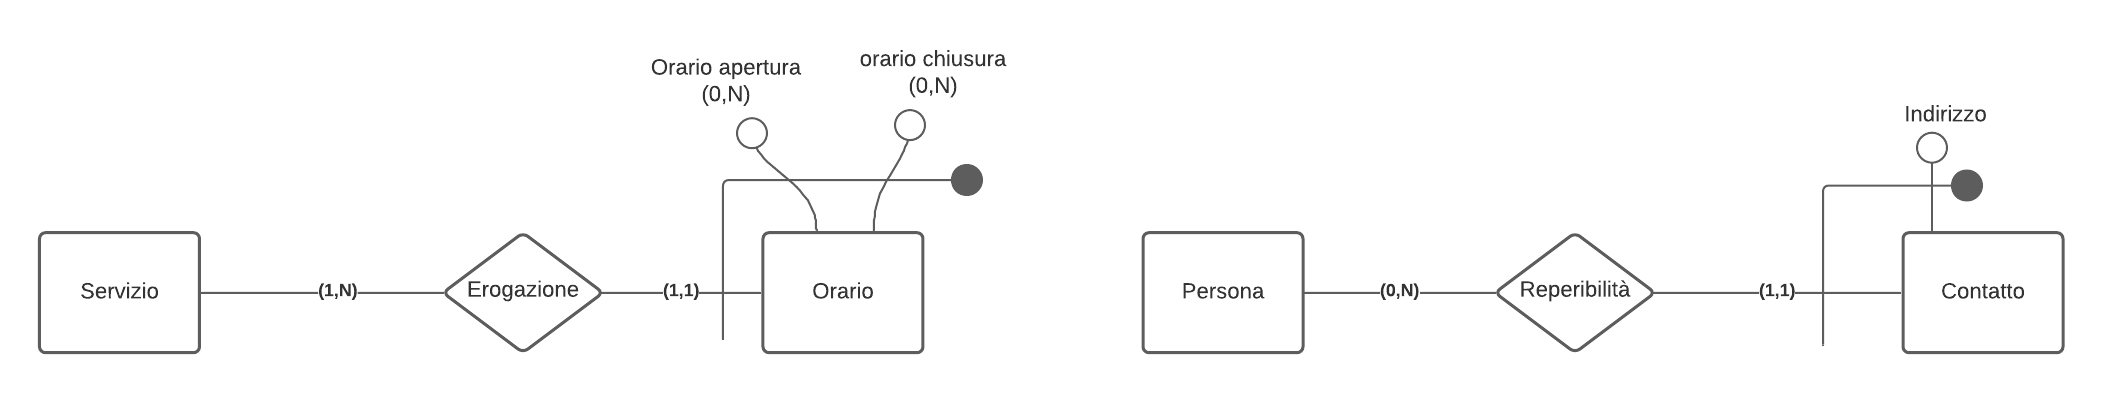
\includegraphics[width=\linewidth]{img/multi_valore.png}

\subsection{Eliminazione delle generalizzazioni}

\paragraph{Cliente}\mbox{}\\
Si accorpano Cliente abituale e cliente occasionale a Cliente. Dato che la quantità di soste è un attributo utile per entrambe le tipologie di cliente. Lo sconto personale sarà invece impostato ad un valore che indica la percentuale di sconto se il cliente è abituale e a NULL se il cliente è occasionale.

\paragraph{Persona}\mbox{}\\
Nelle generalizzazioni di persona, per evitare inutili valori NULL in un eventuale accorpamento \textbf{Persona} viene mantenuta come entità. Questa entità conterrà tutti i dati relativi alla persona e avrà due entità deboli collegate ovvero \textbf{Addetto} e \textbf{Cliente}.

Persona avrà da 0 a 1 \textbf{Cliente} e da 0 a 1 \textbf{Addetto}. Chiaramente ogni \textbf{Cliente}  e \textbf{Addetto} avrà una e una sola persona legata. In \textbf{Addetto} e \textbf{Cliente} posizioneremo i dati relativi a queste due entità come da schema concettuale.

\subsection{Partizionamento/Accorpamento di entità e relazioni}

Le Entità Molo e Imbarcazione condividono l'attributo composto \textbf{Dimensioni}. Le 2 entità possono contenere le stesse dimensioni, quindi gli attributi risultano ridondanti. Viene creata un'entità dimensioni che avrà relazione 1 a molti con Molo ed Imbarcazione.

Inoltre si accorpa l'attributo indirizzo a Marina che avrà quindi gli attributi: Via, provincia, Città, numero civico.

\subsection{Scelta degli identificatori primari}

Le occorrenze di addetto e Cliente vengono identificate dal CF di Persona. 
Orario viene identificato dal nome del servizio e dal marina che lo offre.
Contatto viene identificato dall'indirizzo di contatto e dal CF di persona.

Alcune entità, ovvero: Consumo, Corso, Dimensioni, Molo, Allacciamento, Prenotazione non hanno un identificatore primario concettuale gli daremo quindi un id auto-incrementante.

\subsection{Schema concettuale ristrutturato - Schema logico}
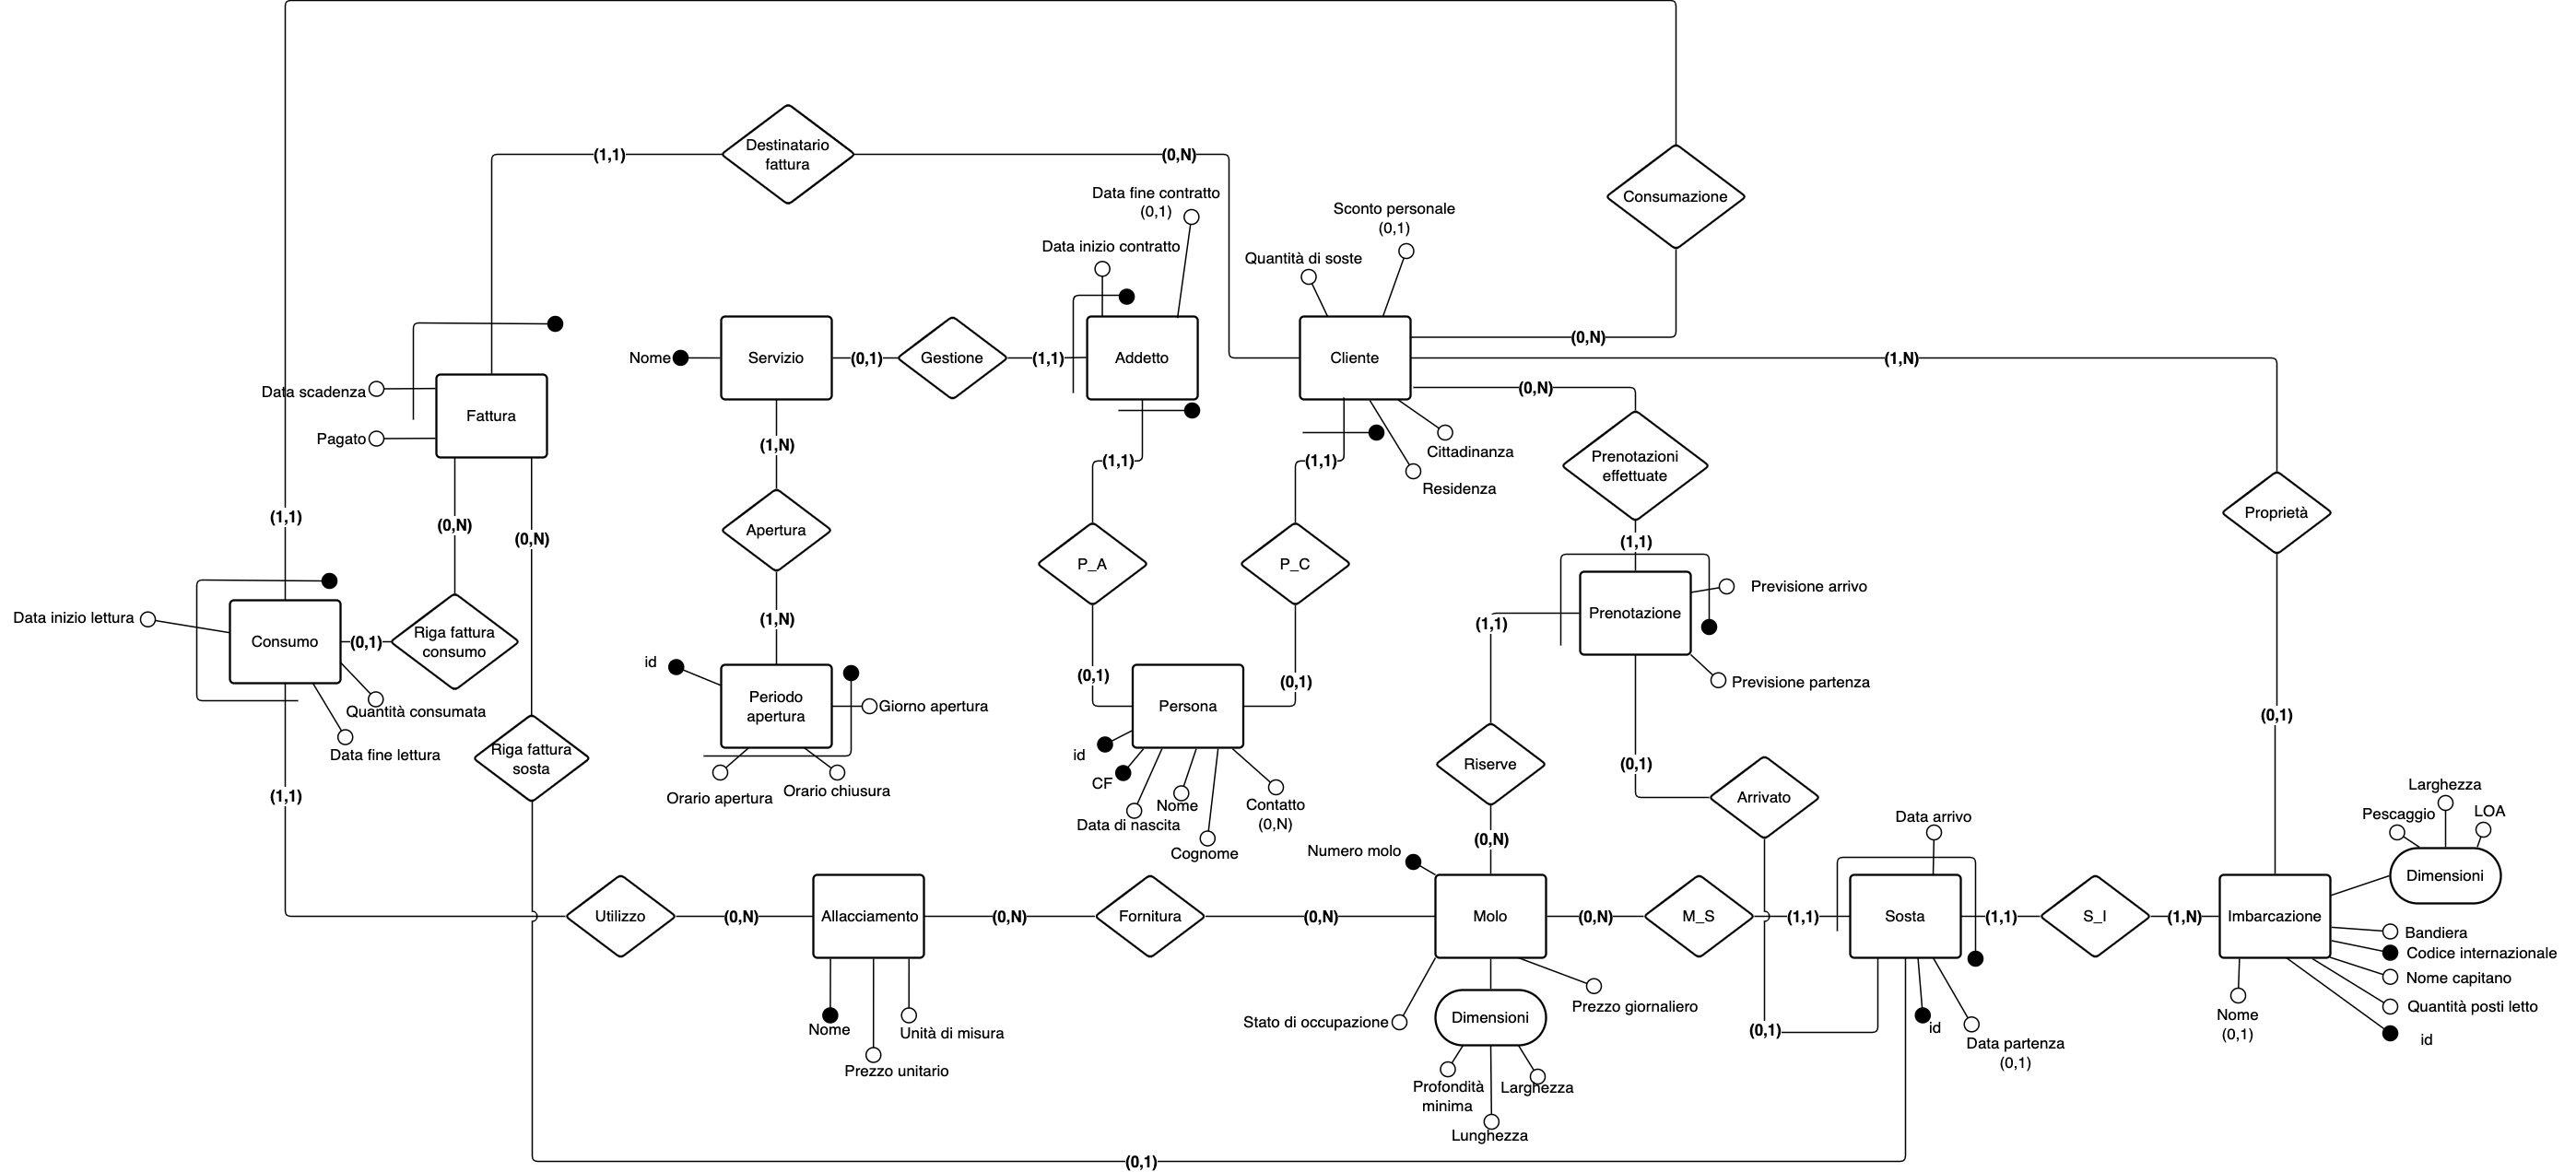
\includegraphics[width=\textwidth]{img/erlogico.png}


\subsection{Descrizione schema relazionale}

Consumo(\underline{id\_consumo},data inizio lettura,data fine lettura,quantità consumata);

Fattura(\underline{codice\_fattura},data\_scadenza,pagato) 

Marina(\underline{coordinate\_geografiche},citta,Nome,quantita moli, numero civico,via,provincia);

Servizio(\underline{marina,Nome});

Orario(\underline{marina,nome\_servizio, orario\_apertura, orario\_chiusura});

Addetto(\underline{persona},data\_inizio\_contratto,data\_fine\_contratto);

Contatto(\underline{persona,indirizzo});

Persona(\underline{CF},data di nascita,nome,cognome);

Molo(\underline{id\_molo},stato di occupazione);

Corso(\underline{id\_corso},prezzo,data inizio,data fine,nome,);

Dimensione(\underline{id\_dimensioni},larghezza,lunghezza,pescaggio);

Allacciamento(\underline{nome},prezzo\_unitario,unita\_di misura);

Prenotazione(\underline{id\_prenotazione},previsione arrivo,previsione\_partenza);

Cliente(\underline{persona},cittadinanza,residenza,marina visitati,data primo arrivo);

Imbarcazione(\underline{codice\_internazionale} ,bandiera,capitano,quantità posti letto, nome);


\subsection{Vincoli di integrità referenziali}

\textbf{Fattura}.cliente -> Cliente.persona\\
\textbf{Addetto}.persona -> Persona.CF\\
\textbf{Cliente}.persona -> Persona.CF\\
\textbf{Molo}.dimensioni -> dimensioni.id\_dimensioni\\
\textbf{Imbarcazione}.dimensioni -> dimensioni.id\_dimensioni\\
\textbf{Servizio}.marina -> Marina.coordinate geografiche\\
\textbf{Contatto}.persona -> Persona.CF\\
\textbf{Orario}.servizio ->Servizio.nome\\
\textbf{Orario}.marina -> Marina.coordinate\_geografiche\\
\textbf{Fattura}.consumo -> Consumo.id\_consumo\\
\textbf{Consumo}.marina -> Marina.coordinate\_geografiche\\
\textbf{Servizio}.addetto -> Addetto.persona\\
\textbf{Prenotazione}.molo -> Molo.id\_molo\\
\textbf{Molo}.marina -> Marina.coordinate\_geografiche\\
